\chapter{Kernel-modulo}

\section{Verso i pattern architetturali}

\dfn{Ereditarietà, parte 2}{
    L'ereditarietà può essere usata per modellare oggetti complessi. Combinando
    l'uso di interfaccie/classi che implementano le interfacce con relazioni di
    combinamento si ottengono modelli di programmazione avanzati.
}

\begin{figure}[h]
    \caption{La classe prisma}
    \begin{center}
        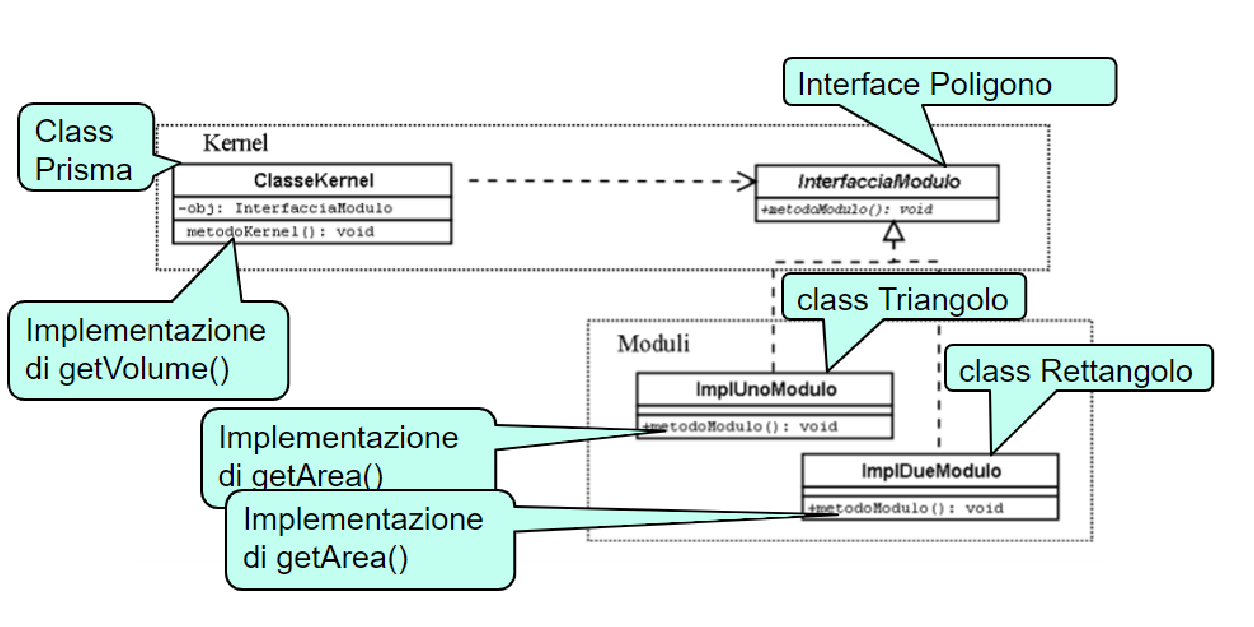
\includegraphics[scale=0.35]{images/Kernel-modulo/Prisma.png}
    \end{center}
\end{figure}
 \nt{
    Questa separazione tra interfaccia e implementazione permette la compilazione
    separata. Inoltre, se si cambia l'implementazione di una classe, non si
    cambia l'interfaccia, quindi non si cambia il codice che usa l'interfaccia.
 }